% Compilare con PDFLaTeX
\documentclass[10pt,final]{siamltex}
\usepackage{graphicx}
\usepackage{latexsym}
\usepackage{amsmath,amssymb}
%\usepackage{gensymb}
\textwidth = 16cm
\usepackage{pstricks}
%\usepackage{subcaption}
\usepackage{algorithm}
\usepackage{algpseudocode}
\usepackage[breakable]{tcolorbox}
\usepackage{doi}
%
\begin{document}
\title{Glomerular filtration rate estimation by a novel binning-less bivariate isotonic statistical regression method}
\author{Sebastian~Giles, Simone~Fiori%
\thanks{S. Giles is with the School of Information and Automation Engineering,
Universit\`{a} Politecnica delle Marche,
Via Brecce Bianche, I-60131 Ancona (Italy).
\newline\indent
S. Fiori is with Dipartimento di Ingegneria dell'Informazione,
Universit\`{a} Politecnica delle Marche,
Via Brecce Bianche, I-60131 Ancona (Italy).
\newline\indent
This draft is dated \today.}}
\maketitle
\def\bbbr{\mathbb{R}}
\def\bbbx{\mathbb{X}}
\def\bbby{\mathbb{Y}}
\def\mdef{{\stackrel{{\mathrm{def}}}{=}}}
% Footnotes in non-numerical fashion
\renewcommand*{\thefootnote}{\fnsymbol{footnote}}
\def\to{\mathbf{\ to\ }}
\setcounter{footnote}{1}
%
%
\begin{abstract}
  Bivariate statistical regression is a method for finding the relationship between unpaired sets of data based on statistic distribution matching. In the present report an  algorithm is proposed to eliminate binning from the previously published procedure. The method is then applied to correlate Glomerular filtration rate (GFR) to serum creatinine concentration. GFR is an important indicator of kidney function, as direct measurement is highly impractical there is considerable interest in developing formulas to estimate it from parameters which are easier to obtain.
\end{abstract}
%
\section{Introduction}\label{intro}
Several real-world phenomena lack accurate mathematical descriptions \cite{strontium, seismic}. In these cases it is not possible to predict the value of a variable by plugging known quantities in to an analytically derived expression, therefore statistical methods must be employed to develop a model of the observed process. The most common set of tools used to infer a functional relationship between variables is regression analysis \cite{control, ts}, here only bivariate regression techniques will be considered. The amount of available data is assumed to be enough to explain the relevant statistical features of the phenomenon underlying the data.

Traditional forms of regression are based on some parametrised function whose graph is made to lie reasonably close to the points making up the experimental dataset. Values for the parameters are typically found using the least squares method \cite{book}.

Isotonic regression allows greater freedom for the regression curve to fit data by constructing a piecewise linear function, described by a lookup table (LUT). Overfitting is avoided by requiring the function to be monotonic, this is obviously also a limit on the process we want to model. Various algorithms can be used to find the LUT values that satisfy a least squares condition \cite{bestchak, pava}.

Statistical bivariate regression (SBR) constitutes an improvement over isotonic regression, its advantages derive from the fact that it relies on finding the relationship between the statistical distributions of the variables. SBR is not based on a least squares method so it does not require data to be associated in ordered pairs, this makes it ideal for correlating two quantities that cannot be both measured on the same individual. The algorithm presented in \cite{fiori} independently estimates the probability density functions (PDF) of the two variables by dividing the dataset ranges into bins and populating LUTs for the relative frequencies, the PDFs are then integrated to obtain the cumulative distribution functions (CDF) which are, or can be licitly adjusted to be, bijective and allow for the regression model to be obtained as the map between values with equal probabilities.

This report describes an alternative algorithm developed to make bivariate statistical regression more versatile and faster over large datasets by entirely avoiding the binning and integration operations.

Glomerular filtration rate (GFR) is used as an indicator of kidney function, as such it is relevant for assessing progression of renal disease, it is also frequently required for evaluating optimal dosage for medications \cite{gfralb, gfrmed}. However, determination of true GFR is time-consuming, costly, and difficult to perform \cite{mgfr, mgfr2}. Thus, there is considerable interest in developing formulas to estimate GFR using simpler parameters such as age, weight, height and sex and values which can be more conveniently measured as part of a blood test.

The present report is organized as follows. Section \ref{blsbr} recalls the notion of bivariate statistical regression and explains the main idea and the details about the proposed binning-less bivariate statistical regression algorithm. Section \ref{cdf} defines and describes the necessary CDF estimation routines. Section \ref{gfr} explains an analysis of the glomerular-filtration-rate (GFR) estimation based on creatinine levels and illustrates such analysis by means of numerical tests performed on a dataset drawn from a study on pediatric patients in mainland China. Section \ref{conclusion} concludes the paper.
%
\section{Binning-less statistical bivariate regression algorithm}\label{blsbr}
%
Given the random variables $X$ and $Y$, for which we expect the existance of a monotonic function $f$ such that $Y=f(X)$, let $D_X \in \mathbb{R}^n$ and $D_Y \in \mathbb{R}^m$ be arrays whose components are realizations of $X$ and $Y$ respectively.

The developed regression algorithm is encapsulated in a function that takes the $D_X$ and $D_Y$ dataset arrays along with an $x$ for which the estimated value of $f(x)$ is returned.

Denoting by $P_X(x)$ and by $P_Y(y)$ the respective CDFs of $X$ and $Y$, we recall from our previous work \cite{fiori,fgl} that
\begin{equation}
  f(x)=P_Y^{-1}(P_X(x)) \text{ if $f$ is monotonically increasing},
\end{equation}
\begin{equation}
  f(x)=P_Y^{-1}(1-P_X(x)) \text{ if $f$ is monotonically decreasing}
\end{equation}
We further recall that, since the modeling solution is not unique, in general, we assumed that the center of mass of the $X$ data corresponds to the center of mass of the $Y$ data.

The regression procedure can be separated into two parts: the evaluation of a CDF and the evaluation of an inverse CDF. In this report the former is handled by the $cdf$ function defined in Algorithm \ref{cdf_algo}, the latter by $invcdf$ defined in Algorithm \ref{invcdf_algo}. Besides the argument for the CDF (or inverse CDF) both procedures require a dataset from which to infer the actual distributions. Algorithm \ref{regression_algo} provides pseudocode for putting the two parts together in the case that a monotonically increasing model is sought. If the model is expected to be monotonically decreasing then \textit{``P''} on Line 3 should be replaced by it's complement \textit{``1-P''}.

\begin{algorithm}
  \caption{Statistical Bivariate Regression}
  \label{regression_algo}
  \begin{algorithmic}[1]
    \Function{statisticalRegression}{$D_X$,$D_Y$, $x_q$}
    \State $P \gets cdf(D_X, x_q)$
    \Comment Evaluate CDF for value $x_q$ in data set $D_X$
    \State $y_q \gets invcdf(D_y, P)$
    \Comment Evaluate inverse CDF for probability $P$ on data set $D_Y$
    \State \Return $y_q$
    \EndFunction
  \end{algorithmic}
\end{algorithm}

\section{Cumulative distribution function estimation algorithm}\label{cdf}
%
This section explains a procedure to estimate the value of the CDF $P(q)$ of a generic random variable for which $n$ realizations are stored as the components of the array $D$.
The main idea to avoid binning is to estimate the cumulative distribution function of the dataset without resorting to an estimate of the probability density function first, this can be done by embracing the definition of CDF itself, which simply leads us to counting the number of realizations that are less than or equal to $q$ and dividing by $n$. The solution shown in algorithm \ref{cdf_algo} expands this idea to allow for a continuos, strictly monotonic interpolation for values which are not included in the original dataset. Please mind that array indexing is 1-based.

\begin{algorithm}
  \caption{Cumulative distribution function estimation}
  \label{cdf_algo}
  \begin{algorithmic}[1]
    \Function{cdf}{$D$, $q$}
    \State $D \gets sort(D)$
    \Comment Dataset is put into ascending order
    \State $n \gets length(D)$
    \State $l \gets 1$
    \State $r \gets n$
    \While {$r - l > 1$}
    \State $m \gets \left \lfloor{(l+r)/2}\right \rfloor$
    \If {$D[m] > q \land D[m]\neq D[l]$}
    \State $r \gets m$
    \Else
    \State $l \gets m$
    \EndIf
    \EndWhile


    \While{$D[r] = D[l]$}
    \State $l \gets l - 1$
    \EndWhile

    \While {$r < n \land D[r] = D[r+1]$}
    \State $r \gets r + 1$
    \EndWhile
    \State $d \gets (q-D[l])/(D[r]-D[l])$
    \State $p \gets (l + d \cdot (r - l))/n $

    % trim out of range interpolations
    \If {$p<0$}
    \State {$p\gets0$}
    \ElsIf {$p>1$}
    \State {$p\gets1$}
    \EndIf

    \State \Return $p$
    \EndFunction
  \end{algorithmic}
\end{algorithm}

Here are a few comments about Algorithm \ref{cdf_algo}:
\begin{itemize}
  \item \textbf{Line 2}: The algorithm is notably simplified by sorting $D$ into ascending order.
  \item \textbf{Lines 4--13}: This part is essentially a binary search for $q$ in array $D$. The loop starts with indexes $l$ and $r$ as the extremes of $D$ and ends with $l$ as the index of the last value less than $q$, and $r$ as that of the first value greater than $q$. The only exception that may occur is handled in lines 14--16.
  \item \textbf{Line 8}: Making sure that $D[m]\neq D[l]$ is needed to stop $l$ and $r$ converging to $1$ and $2$ respectively, in the case that $q$ is smaller than all elements in $D$.
  \item \textbf{Lines 14--16}: This loop is needed to fix $l$ in the case it converges to $n-1$ as a consequence of $q$ being greater than all values in $D$.
  \item \textbf{Lines 17--19}: The previous operations already guarantee that $l$ is the last index for the value $D[l]$, this means there are $l$ elements in $D$ which are less than or equal to $D[l]$. This loop finds $r$, the count of elements that are less than or equal to $D[r]$.
  \item \textbf{Lines 20--21}: $P(D[l])$ can be estimated by $l/n$ whilst $P(D[r])$ can be estimated by $r/n$, $P(q)$ is obtained via linear interpolation.
  \item \textbf{Lines 22--26}: These checks limit the CDF for values outside the range of $D$.
\end{itemize}
%

\begin{algorithm}
  \caption{Inverse Cumulative distribution function estimation}
  \label{invcdf_algo}
  \begin{algorithmic}[1]
    \Function{invcdf}{$D$,$P_q$}
    \State $D \gets sort(D)$
    \Comment Dataset is put into ascending order
    \State $n \gets length(D)$
    \State $p \gets P_q \cdot n$
    \State $r \gets  \left \lceil{p}\right \rceil$
    \If {$r=0$}
    \State {$r\gets1$}
    \EndIf
    \State $l \gets r$

    \While{$r < n \land D[r] = D[r+1]$}
    \State $ r \gets r + 1$
    \EndWhile

    \While {$l > 1 \land D[l - 1] = D[l]$}
    \State $l \gets l - 1$
    \EndWhile

    \If {$l = 1$}
    \State $l \gets r$
    \State $r \gets r+1$
    \While {$r < n \land D[r] = D[r+1]$}
    \State $r \gets r + 1$
    \EndWhile
    \Else
    \State $ l \gets l - 1$
    \EndIf

    \State $d \gets (p-l)/(r-l) $
    \State $q \gets D[l] + d \cdot (D[r]-D[l])$

    \State \Return $q$
    \EndFunction
  \end{algorithmic}
\end{algorithm}

Evaluation of the inverse CDF is based on the same principle only applied in reverse: the input argument is a probability, it is multiplied by $n$ and rounded to an integer $r$. If the dataset $D$ is sorted, then there will be $r$ values less than or equal to $D[r]$. Algorithm \ref{invcdf_algo} allows for a continuos, strictly monotonic interpolation to yield values which are not included in the original dataset.
Here are a few comments about Algorithm \ref{invcdf_algo}:
\begin{itemize}
  \item \textbf{Line 2}: The algorithm is notably simplified by sorting $D$ into ascending order.
  \item \textbf{Line 4}: The input probability is denormalised into the range $[0, n]$.
  \item \textbf{Lines 5--9}: $r$ and $l$ take the value of $p$ rounded to the next integer to be used as an index, this also requires $r$ and $l$ to be non-zero.
  \item \textbf{Lines 10--12}: $r$ is made to point to the last occurence of the smallest value whose CDF is greater than the requested probability.
  \item \textbf{Lines 13--15, 20}: $l$ is made to point to the last occurence of the greatest value whose CDF is less than the requested probability.
  \item \textbf{Lines 16--22}: Alignments are made to allow interpolation for small probabilities.
  \item \textbf{Lines 20--21}: $P^{-1}(l/n)$ can be estimated by $D[l]$ whilst $P^{-1}(r/n)$ can be estimated by $D[r]$, nearby values are obtained via linear interpolation.
\end{itemize}
%

\begin{tcolorbox}[colback=gray!30,%gray background
  colframe=black,% black frame colour
  width=\dimexpr\linewidth-2\fboxrule\relax,
  arc=3mm, auto outer arc,
  breakable
  ]
  \underline{\textsc{Small numerical example}}: Let $X=[2,3,5,5,6,6,7,9]$, $Y=[6,7,10,10,11,11,11,12,15,20]$, i.e., $n=8$, $m=10$. The actual underlying model is $f(x)=2x+2$. Note that the data aren't paired. Both arrays are already sorted for simplicity. Let the query point be $q=4$, we expect $y_q\approx10$.

Let's first estimate $P_X(4)$: the $cdf$ algorithm will find $l=2$ and $r=4$. It then computes the linear interpolation:
  %
  \begin{equation*}
    d = \tfrac{q-X[l]}{X[r]-X[l]} = \tfrac{4-3}{5-3} = 0.5
    \quad\quad
    P_X(4)=\tfrac{l+d\cdot(r-l)}{n}=\tfrac{2+0.5\cdot(4-2)}{8}=0.375
  \end{equation*}

Now it's time to estimate $P^-1_Y(0.375)$: the $invcdf$ algorithm will find $p = 0.375  m=3.75$, $r=4$ and $l=2$. By linear interpolation, it then finds
    %
    \begin{equation*}
      d = \tfrac{p-l}{r-l} = \tfrac{3.75-2}{4-2} = 0.875
    \end{equation*}
    \begin{equation*}
      P^-1_Y(0.375)=D[l]+d\cdot(D[r]-D[l])=7+0.875\cdot(10-7)=9.625
    \end{equation*}
\end{tcolorbox}
%
\section{Application to glomerular filtration rate estimation}\label{gfr}

\begin{figure}[ht]
  \centering
  \makebox[\textwidth][c]{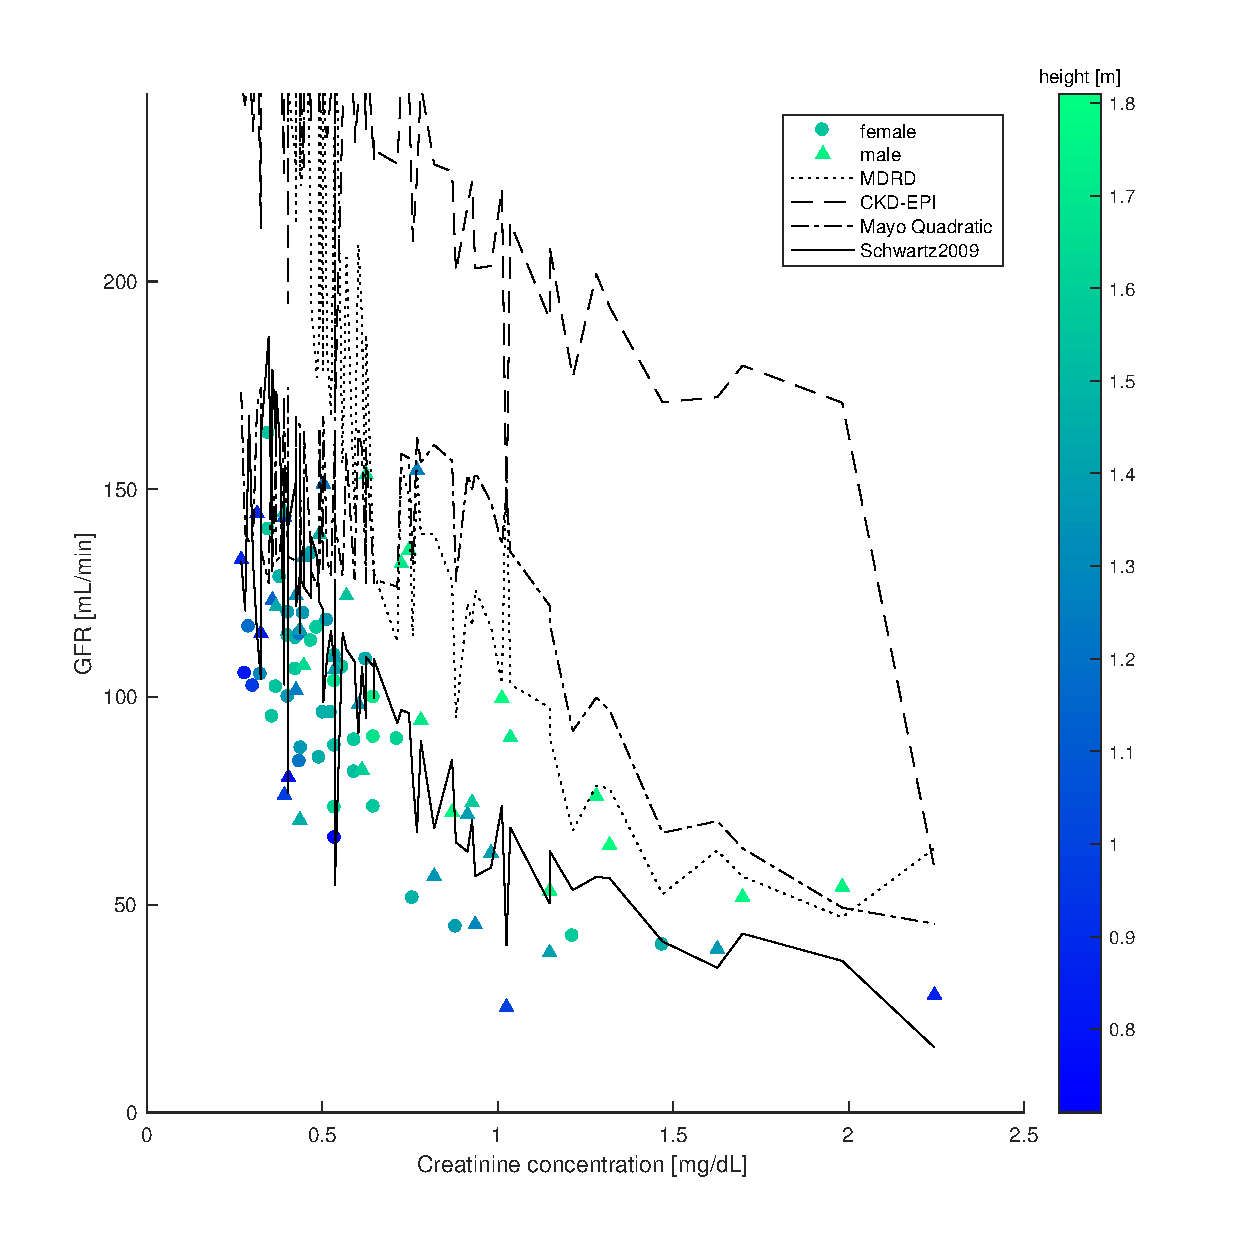
\includegraphics[scale=0.6]{figures/equations}}
  \caption{Comparison of predictions made using the different equations \cite{gfr}.}
  \label{equations}
\end{figure}

Existing multivariate formulas for GFR estimation have been compared and validated in \cite{gfr} over a dataset of 86 Chinese children and adolescents aged 1 through 18, authors of this research have included the dataset with their publication. The most effective was found to be the Schwartz2009 equation \cite{schwartz} (from here on in this report units for $eGFR$ and Serum Creatinine concentration will be mL/min and mg/dL respectively, height is in meters):
$$ eGFR = 41.3 \cdot \frac{height}{Serum Creatinine}.$$

Over said data we also computed estimations using the other three widely employed formulas that follow and compared them with the results of the Schwartz2009 estimation. The MDRD 4-variable equation \cite{MDRD}:
$$ eGFR = 186 \cdot Serum Creatinine^{-1.154}\cdot Age^{-0.203} \cdot [1.2010 \text{ if Black}] \cdot [0.742 \text{ if Female}].$$

The CKD-EPI formula \cite{ckdepi} ($SCr$ is serum creatinine, $k$ is $0.7$ for females and $0.9$ for males, $a$ is $−0.329$ for females and $−0.411$ for males):
$$ eGFR = 141 \cdot min(SCr/k,1)^a\cdot max(SCr/k,1)^{-1.209}\cdot0.993^{Age}\cdot [1.018 \text{ if Female}] \cdot [1.159 \text{ if Black}].$$

The Mayo Quadratic formula \cite{mayo} (if $SCr$ is less than $0.8 mg/dL$, use $0.8 mg/dL$ for $SCr$):
$$eGFR = exp(1.911+\frac{5.249}{SCr}-\frac{2.114}{SCr^2}-0.00686\cdot Age - [0.205 \text{ if Female}])$$

Looking at Figure \ref{equations} it is clear that the Schwartz2009 equation outperforms all of the other functions.

In order to apply SBR we must first assess the existance of a single dominant variable, this was clearly found to be the serum creatinine concentration, other variables used to estimate GFR are age and height, their effect however is marginal, as the scatter plots in Figure \ref{recessive} reveal no strong statistical features.

\begin{figure}[ht]
  \centering
  \makebox[\textwidth][c]{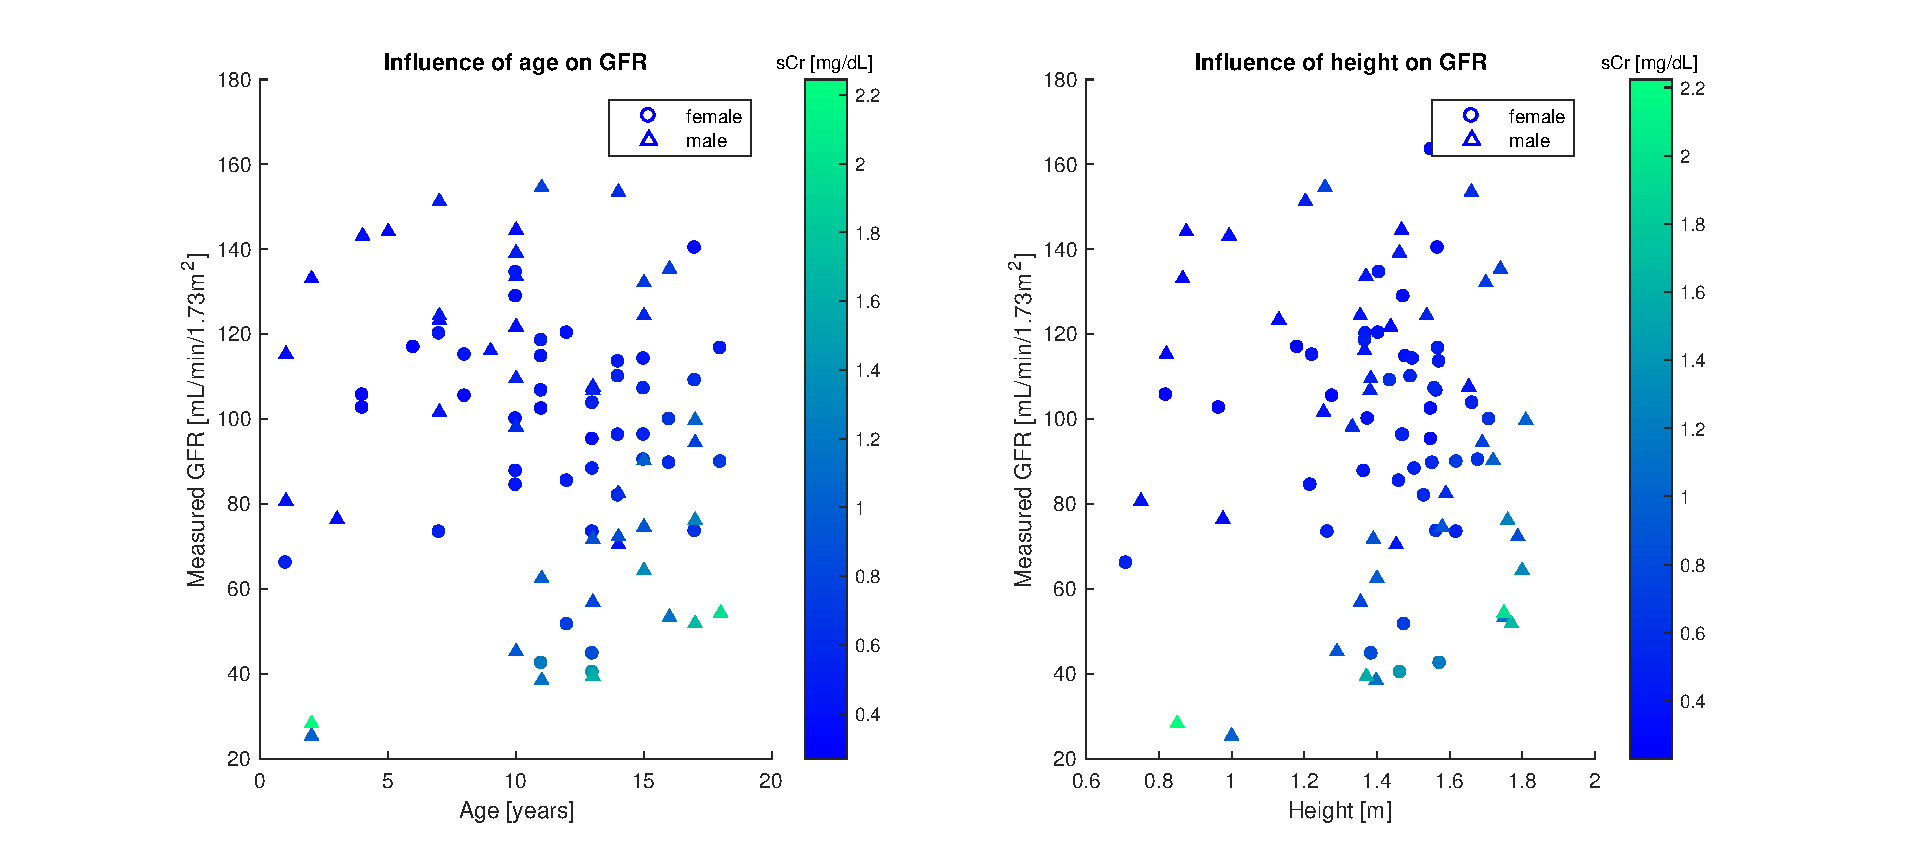
\includegraphics[scale=0.6]{figures/recessive}}
  \caption{Plotting GFR as a function of Age or Height does not show very strong correlation.}
  \label{recessive}
\end{figure}

As SBR generates a univariate model, for the sake of the comparison, the Schwartz2009 equation was simplified to be independent of height, this was done by replacing the variable with a constant equal to the mean height of all individuals in the dataset. This model was plotted in dark blue in Figure \ref{regression}, along with the datapoints, the regression curve obtained by SBR using the Numerical-Algebraic Neural System (NANS) method explained in \cite{fiori} and that obtained using the binning-less method described in Section 2.

\begin{figure}[ht]
  \centering
  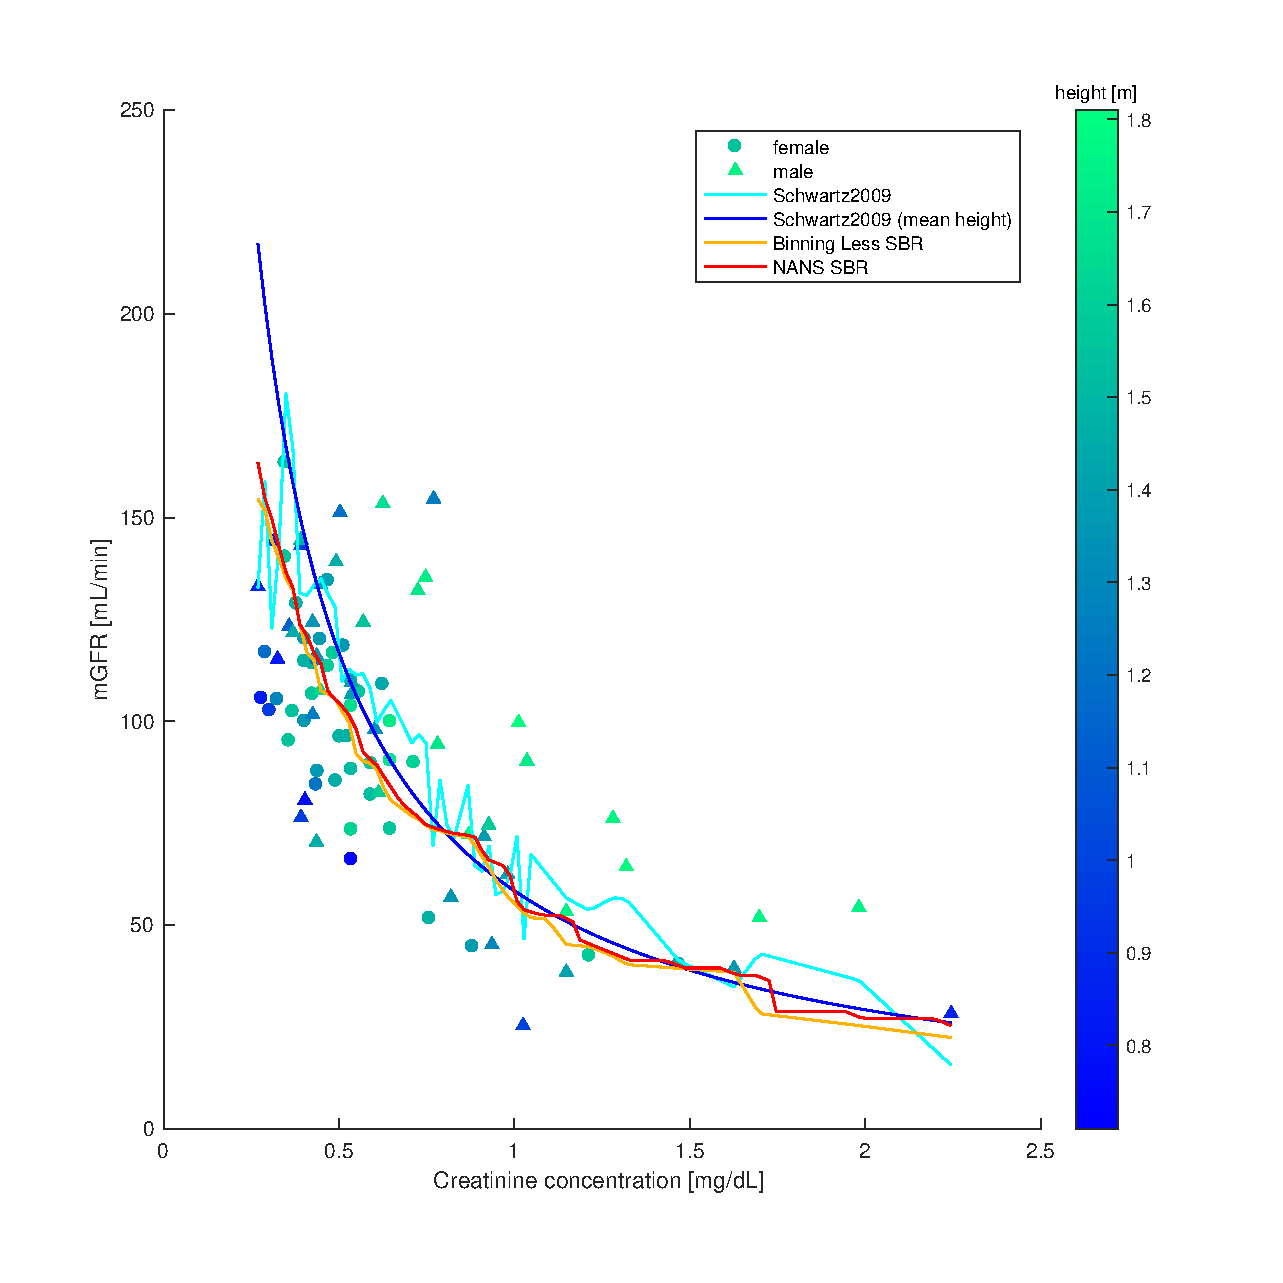
\includegraphics[scale=0.6]{figures/regression}
  \caption{Data set with overlaid regression and estimation curves. }
  \label{regression}
\end{figure}

The four curves in Figure \ref{regression} are compared on prediction performance, i.e. how close along the vertical axis the regression functions come to the measured data, an index (MSE) for this is calculated by averaging the squares of all errors. The Schwartz2009 curve has a low MSE as it also takes height into account, the SBR regressions are both better as they we're obtained from the same data we are now validating them on, anyway this shows that SBR is very effective at fitting data.
Comparisons were also made to evaluate the generality of the models obtained, a good way to evaluate this is by calculating the roughness index
$$ R = \sqrt{\sum_{i=3}^{n}{\frac{(y_i-2y_{i-1}+y_{i-2})^2}{n-2}}}.$$
$R$ is the root mean square of the second order differences of the sequence $y_n$, so $R$ increases with sharp changes in slope. To be useful, the $y_n$ values have to be sorted in some significant manner, in our case, for each model to be evaluated, $y_n$ assumes the values interpolated at increasing, equally spaced values of creatinine concentration. An index similar to $R$ is also used in \cite{bishop} to prevent overfitting.
The value of $R$ is expected to be greater for irregular curves and indeed it is close to zero for the simplified Schwartz2009 model (independent of height), which is essentially a hyperbola, graph of a smooth function, while it is very high for the Schwartz2009 curve, as we are including the effect of a second independent variable (which does contribute to ordering $y_n$)
The $MSE$ and $R$ indices can be read in the table of figure \ref{table}.

\begin{figure}[ht]
  \centering
  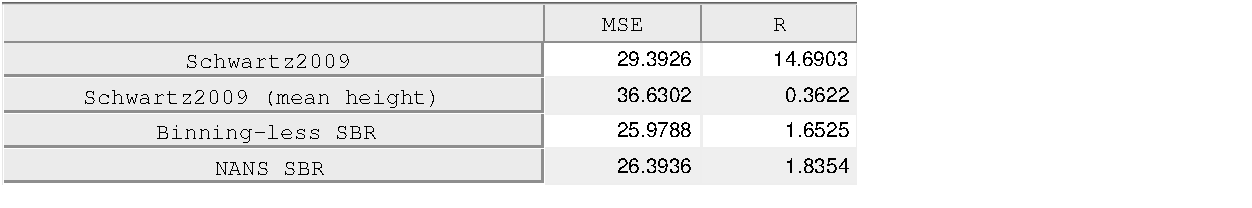
\includegraphics[scale=0.6]{figures/table}
  \caption{Mean squared error with respect to measured GFR (MSE) and roughness(R) for the four estimation models. }
  \label{table}
\end{figure}

\section{Conclusions}\label{conclusion}
%
The aim of the present paper is to discuss the bivariate statistical regression method and to provide an improved algorithm which does not rely on binning for the steps which require computation of the estimated distribution functions. The new algorithm was then compared to the original bivariate statistical regression based on numerical-algebraic neural systems in the application to a real-world data set. The comparison proved an all-round improvement in the new method, which, aside from being more efficient, yields a closer fit and a smoother curve.
%
\begin{thebibliography}{99}
  %
  \bibitem{fiori} S. Fiori, ``Fast statistical regression in presence of a dominant independent variable'', \textit{Neural Computing and Applications}, Vol. 22, No. 7, pp. 1367 -- 1378, 2013
  \bibitem{bishop} C.M. Bishop, ``Training with noise is equivalent to Tikhonov regularization'', \textit{Neural Computation}, Vol. 7, No. 1, pp. 108 -- 116, 1995
  \bibitem{fgl} S. Fiori, T. Gong and H.K. Lee, ``Bivariate nonisotonic statistical regression by a lookup table neural system'', \textit{Cognitive Computation}, Vol. 7, No. 6, pp. 715 -- 730, 2015
  \bibitem{gfr} K. Zheng, M. Gong, Y. Qin, H. Song, X. Shi, Y. Wu, F. Li and X. Li, ``Validation of glomerular filtration rate-estimating equations in Chinese children'', \textit{PLoS ONE}, Vol. 12, No. 7, pp. e0180565 (\doi{10.1371/journal.pone.0180565}), 2017
  \bibitem{strontium}Strontium Isotope Stratigraphy: LOWESS Version 3: Best Fit to the Marine Sr‐Isotope Curve for 0–509 Ma and Accompanying Look‐up Table for Deriving Numerical Age
J. M. McArthur, R. J. Howarth, and T. R. Bailey
The Journal of Geology 2001 109:2, 155-170
\bibitem{seismic}Dengliang Gao (2004). ”Texture model regression for effective feature discrimination: Application to seismic facies visualization and interpretation.” GEOPHYSICS, 69(4), 958-967.
\bibitem{schwartz}G.J. Schwartz, A. Muñoz, M.F. Schneider, R.H. Mak, F. Kaskel, B.A. Warady and S.L. Furth, "New equations to estimate GFR in Children with CKD", Journal of the American Society of Nephrology, Vol. 20, No. 3, pp. 629 – 637, March 2009
\bibitem{control}R. E. KOPP and R. J. ORFORD.  "LINEAR REGRESSION APPLIED TO SYSTEM IDENTIFICATION FOR ADAPTIVE CONTROL SYSTEMS", AIAA Journal, Vol. 1, No. 10 (1963), pp. 2300-2306.
\bibitem{ts}Masry, E. (1996), MULTIVARIATE LOCAL POLYNOMIAL REGRESSION FOR TIME SERIES:UNIFORM STRONG CONSISTENCY AND RATES. Journal of Time Series Analysis, 17: 571–599. doi:10.1111/j.1467-9892.1996.tb00294.x
\bibitem{book}Harrell, Frank E. Regression modeling strategies: with applications to linear models, logistic and ordinal regression, and survival analysis. Springer, 2015.
\bibitem{bestchak}Best, M.J.; Chakravarti N. (1990). "Active set algorithms for isotonic regression; a unifying framework". Mathematical Programming. 47: 425–439. doi:10.1007/BF01580873
\bibitem{pava}Mair, Patrick and Hornik, Kurt and de Leeuw, Jan (2009) Isotone Optimization in R: Pool-Adjacent-Violators
 Algorithm (PAVA) and Active Set Methods. Journal of Statistical Software, 32 (5). pp. 1-24. ISSN 1548-7660
\bibitem{gfralb}Association of estimated glomerular filtration rate and albuminuria with all-cause and cardiovascular mortality in general population cohorts: a collaborative meta-analysis, In The Lancet, Volume 375, Issue 9731, 2010, Pages 2073-2081, ISSN 0140-6736, https://doi.org/10.1016/S0140-6736(10)60674-5.
(http://www.sciencedirect.com/science/article/pii/S0140673610606745)
\bibitem{gfrmed}Jagbir Gill, Rhonda Malyuk, Ognjenka Djurdjev, Adeera Levin; Use of GFR equations to adjust drug doses in an elderly multi-ethnic group—a cautionary tale, Nephrology Dialysis Transplantation, Volume 22, Issue 10, 1 October 2007, Pages 2894–2899, https://doi.org/10.1093/ndt/gfm289
\bibitem{mgfr}Inga Soveri, Ulla B. Berg, Jonas Björk, Carl-Gustaf Elinder, Anders Grubb, Ingegerd Mejare, Gunnar Sterner, Sten-Erik Bäck, Measuring GFR: A Systematic Review, In American Journal of Kidney Diseases, Volume 64, Issue 3, 2014, Pages 411-424, ISSN 0272-6386, https://doi.org/10.1053/j.ajkd.2014.04.010.
(http://www.sciencedirect.com/science/article/pii/S0272638614007343)
Keywords: Glomerular filtration rate (GFR); glomerular filtration rate (GFR) measurement; renal function; clearance marker; accuracy
\bibitem{mgfr2}Clearance and beyond: the complementary roles of GFR measurement and injury biomarkers in acute kidney injury (AKI)
Zoltán H. Endre, John W. Pickering, Robert J. Walker
American Journal of Physiology - Renal Physiology Published 29 September 2011 Vol. 301 no. 4, F697-F707 DOI: 10.1152/ajprenal.00448.2010
\bibitem{MDRD}Levey AS, Bosch JP, Lewis JB, Greene T, Rogers N, Roth D, et al. A More Accurate Method To Estimate Glomerular Filtration Rate from Serum Creatinine: A New Prediction Equation. Ann Intern Med. 1999;130:461–470. doi: 10.7326/0003-4819-130-6-199903160-00002
\bibitem{ckdepi}Levey AS, Stevens LA, Schmid CH, et al. A New Equation to Estimate Glomerular Filtration Rate. Annals of internal medicine. 2009;150(9):604-612.
\bibitem{mayo}Rule AD, Larson TS, Bergstralh EJ, Slezak JM, Jacobsen SJ, Cosio FG (December 2004). "Using serum creatinine to estimate glomerular filtration rate: accuracy in good health and in chronic kidney disease". Annals of Internal Medicine. 141 (12): 929–37.


  %
\end{thebibliography}
\end{document}
